\entry{Semana del 21/04/2025}
\section{Miércoles 23/04}
\subsection*{Resumen rápido}
\begin{itemize}
	\item Hicimos los nuevos cambios al diseño de la carcasa del sensor para mandarlo a imprimir.
	\item Pablo comentó el Lunes de la semana pasada que había comprado los alambres de cobre y que llegaron el Miércoles, sin embargo los diámetros no eran los especificados por MercadoLibre (0.25 y 0.35 mm por 500 g). Realizó la devolución con el reembolso correspondiente (que completaron hoy), y proseguiremos intentando comprarlos presencialmente.
	\item Respecto al alambre de acero vamos a usar de momento uno de acero que ya había en el Laboratorio bastante rígido, de unos 0.5 mm de diámetro.
\end{itemize}

\subsection*{Nuevo diseño de la carcasa}
Los cambios que se hicieron fueron principalmente reducir aún más el tamaño de la cabeza del sensor y la altura de la parte de abajo. Además se agregó un adaptador a una de las mitades que permita conectarlo al soporte de un tornillo micrométrico mediante dos tornillos M4. Además se agregaron salientes en la parte de arriba para poder conectar las dos mitades mediante también tornillos M4, y en la sección inferior se cambio el cilindro por un rectángulo con otros dos agujeros que permitan terminar de conectar ambas mitades. Además se aumentó el diámetro del canal para el cable de cobre que se había cerrado en la impresión anterior.

A continuación se muestra el modelo final.

\begin{figure}[!ht]
	\begin{minipage}[c]{0.5\textwidth}
			\begin{subfigure}{\textwidth}
					\centering
					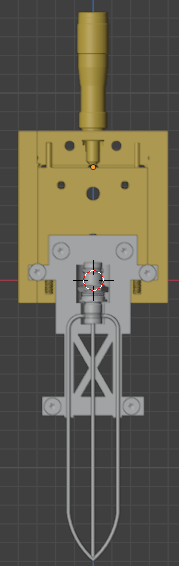
\includegraphics[height=1.30253508\textwidth]{Figures/21_04_2025/Vista_frontal_conector_y_sensor}
					\captionsetup{width=0.8\textwidth}
					\subcaption{Vista frontal.}
				\end{subfigure}
		\end{minipage}\begin{minipage}[c]{0.49\textwidth}
			\begin{subfigure}{\textwidth}
					\centering
					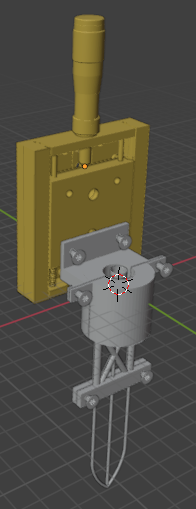
\includegraphics[height=1.30253508\textwidth]{Figures/21_04_2025/Vista_3_4_conector_y_sensor}
					\captionsetup{width=0.8\textwidth}
					\subcaption{Vista 3/4.}
				\end{subfigure}
		\end{minipage}
	\caption{Distintas vistas del nuevo modelo de la carcasa del sensor junto con el tornillo micrométrico.} % para 
	\label{fig:Prototipo_4_carcasa_sensor}
\end{figure}

El tornillo y el soporte del mismo son de la marca Newsport, modelos BM17-25 y M-UMR8-25 respectivamente.

Algunos pensamientos para el próximo prototipo: 
\begin{itemize}
	\item Agregar un tope en la parte del BNC (reducir el cilindro) para que una vez cerrado no se pueda salir por arriba tirando del cable.
	\item Bajar los salientes para los tornillos de arriba que conectan ambas mitades para que queden al ras con el conector al tornillo.
\end{itemize}



\section{Viernes 25/04}
\subsection*{Resumen rápido}
\begin{itemize}
	\item Recibimos las impresiones del nuevo modelo de la carcasa.
	\item Diseñamos una forma de montar el tornillo micrométrico a un perfil para mandarlo a imprimir también en 3D.
	\item Se realizó un inventario de los componentes electrónicos presentes en el Laboratorio y se confeccionó la lista de compras para los faltantes en ELEMON. 
\end{itemize}

\subsection*{Nuevo modelo impreso.}
Recibimos las nuevas impresiones para la carcasa del sensor, que resultaron ser de las medidas especificadas, conectando perfectamente con los agujeros del soporte del tornillo micrométrico. Una cosa a notar es que los demás agujeros para los tornillos M4 se redujeron un poco, aunque igual se pudieron usar, pero casi sin juego. % ligeramente. 

A continuación algunas fotos: 

\begin{figure}[!ht]
	\begin{minipage}[c]{0.5\textwidth} % 34235
			\begin{subfigure}{\textwidth}
				\centering
				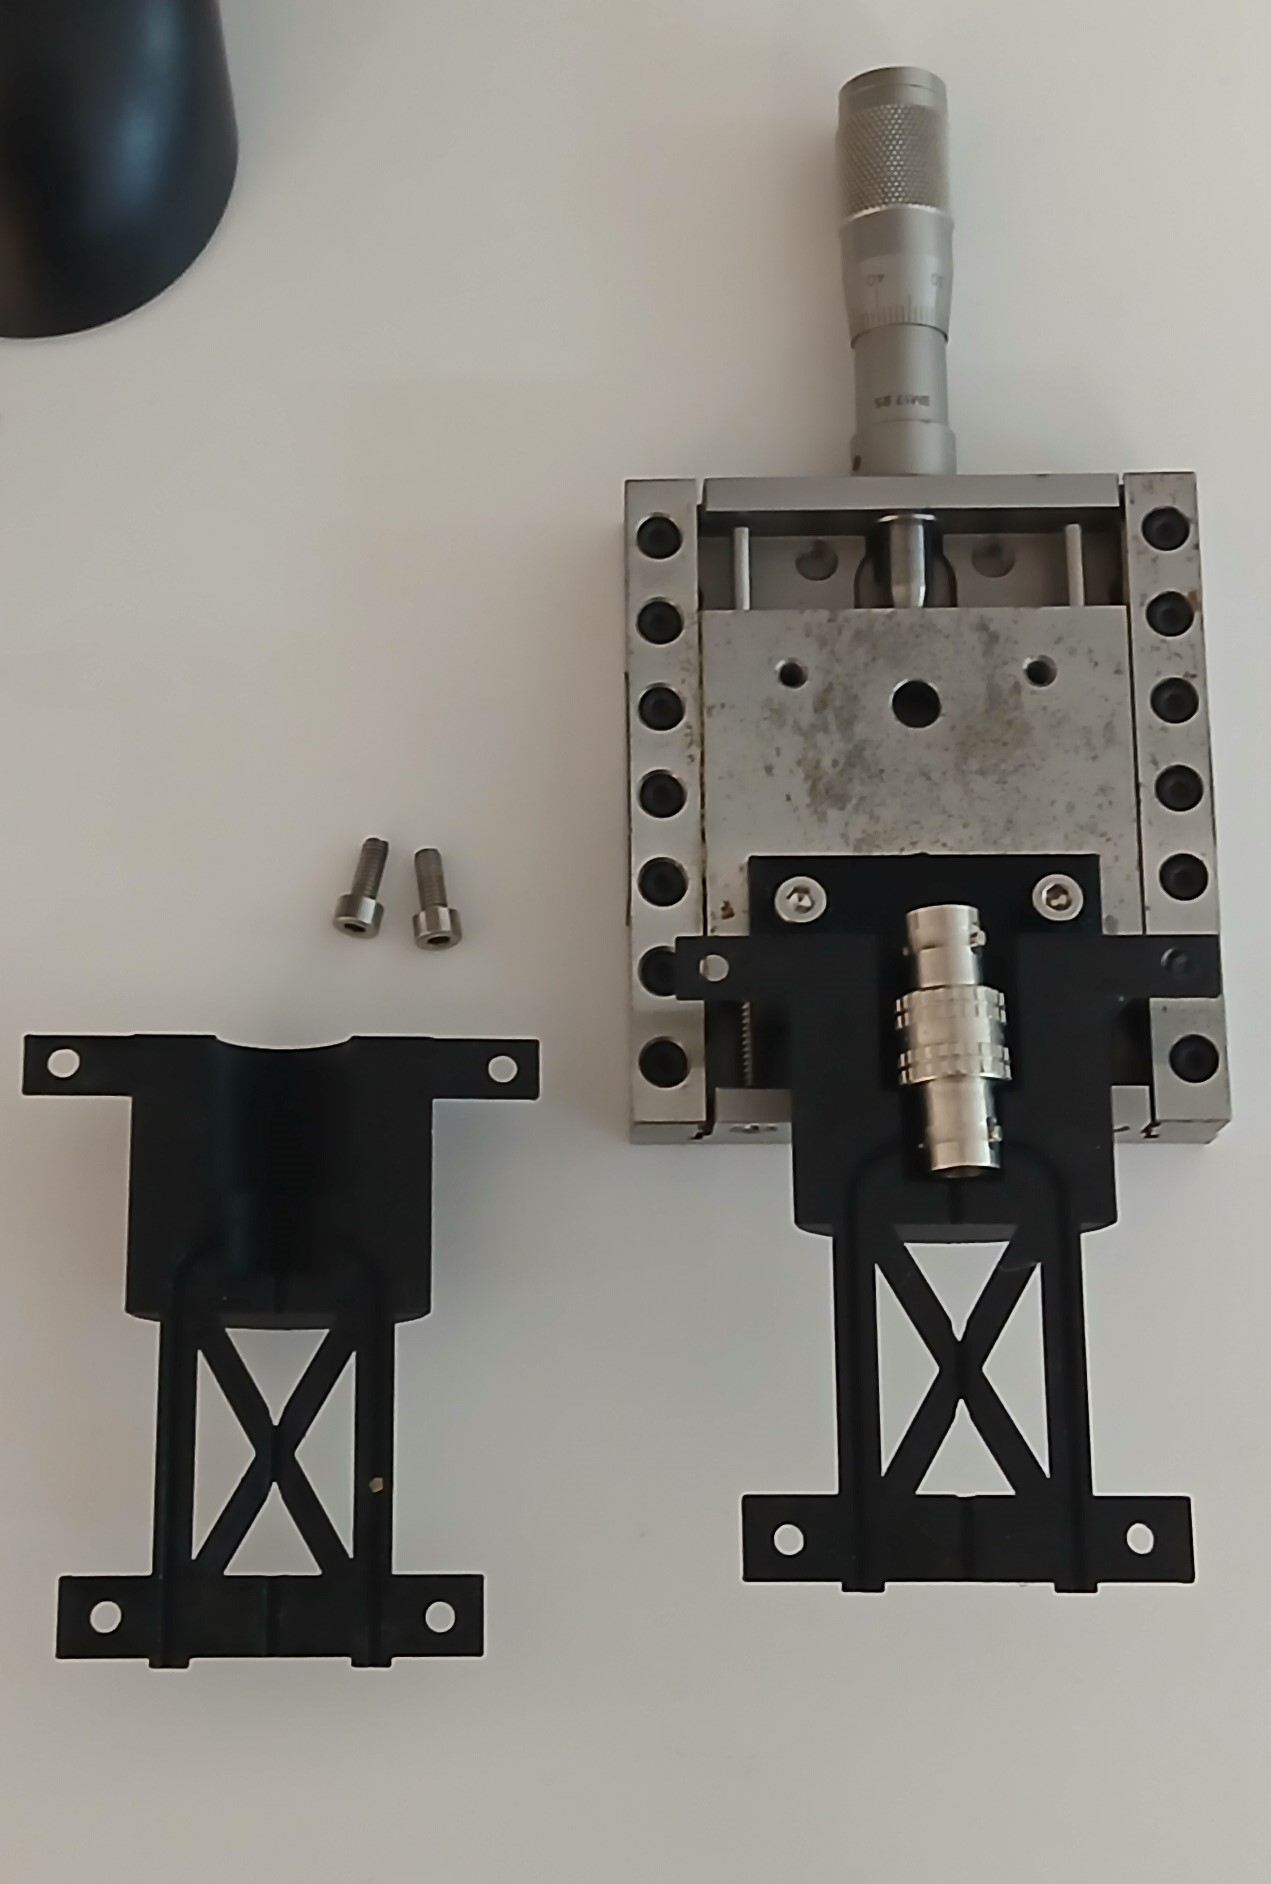
\includegraphics[height=250pt]{Figures/21_04_2025/Vista_frontal_impresa.jpg}
				\captionsetup{width=0.8\textwidth}
				\subcaption{Vista frontal completa.}
			\end{subfigure}
		\end{minipage}\begin{minipage}[c]{0.2\textwidth} % 3249 #  
			\begin{subfigure}{\textwidth}
				\centering
				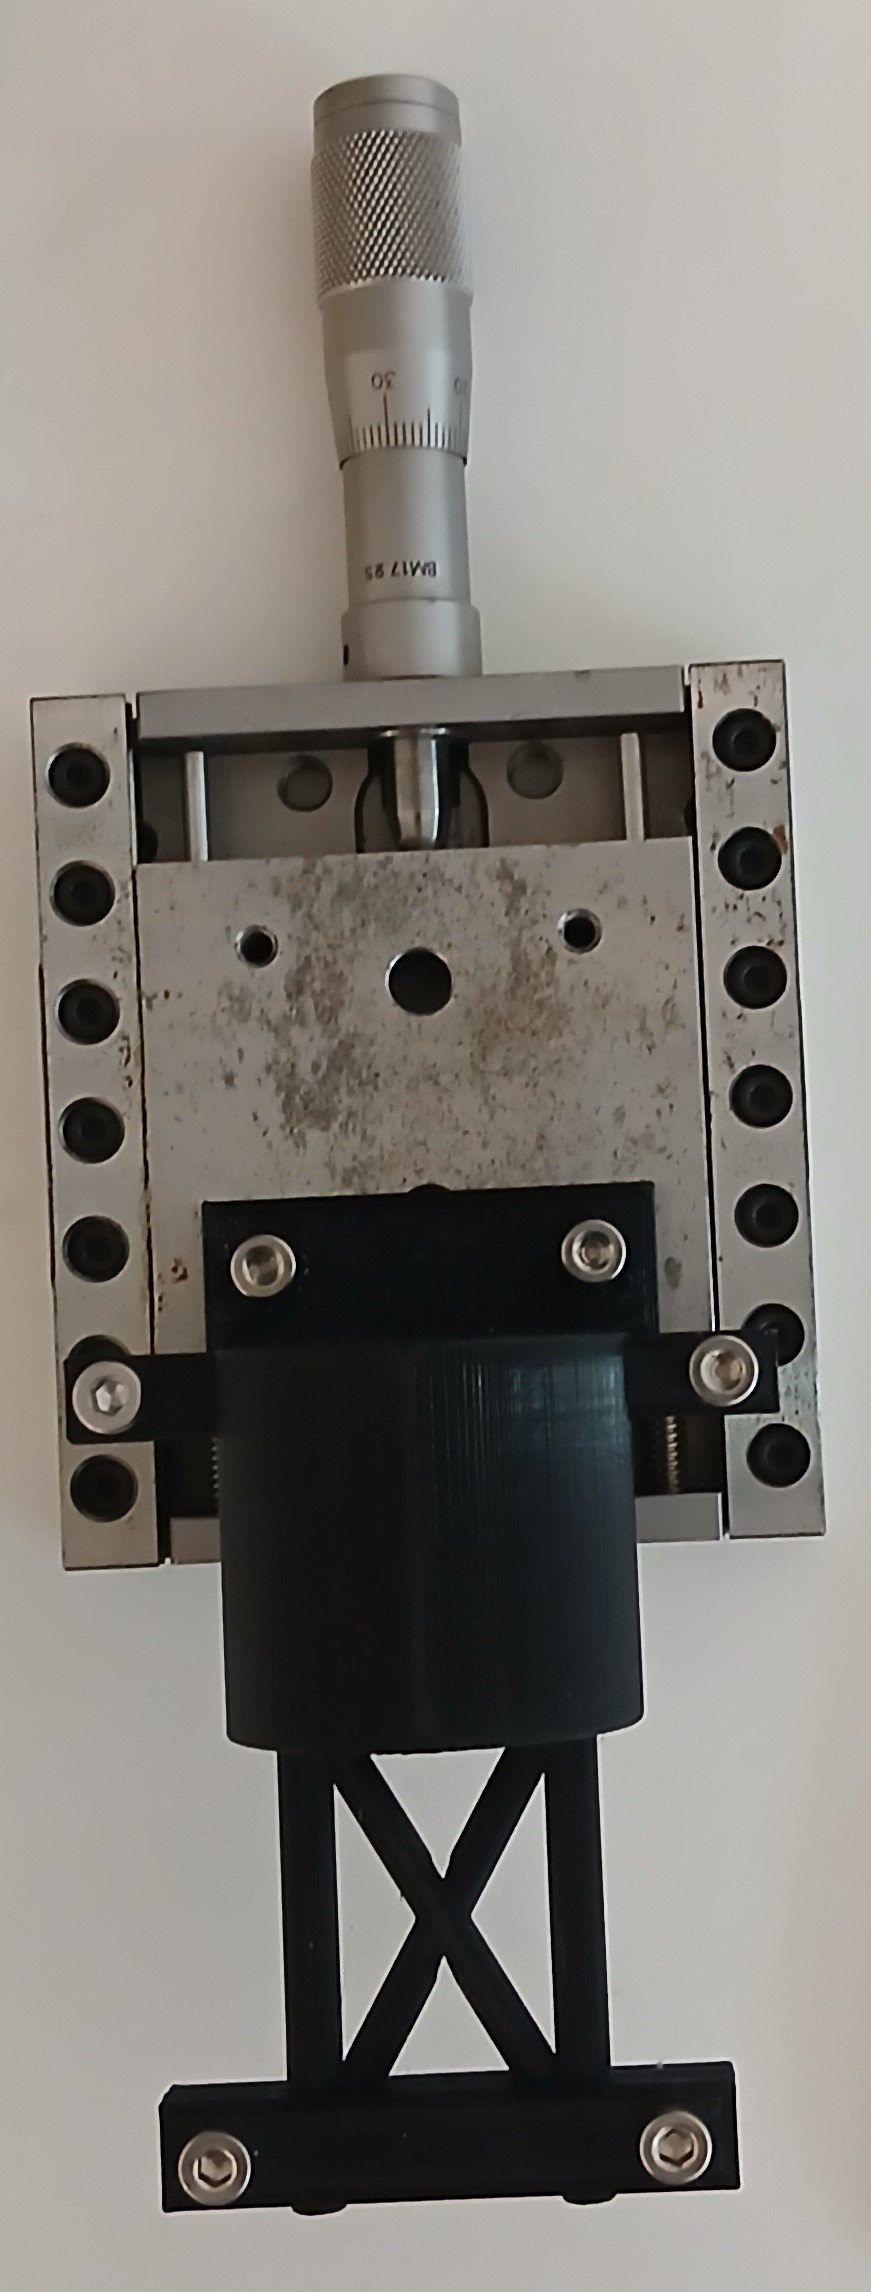
\includegraphics[height=250pt]{Figures/21_04_2025/Vista_frontal_completa_imrpesa.jpg}
				\captionsetup{width=0.8\textwidth}
				\subcaption{Vista frontal.}
			\end{subfigure}
		\end{minipage}\begin{minipage}[c]{0.293054\textwidth} % 3249 
			\begin{subfigure}{\textwidth}
				\centering
				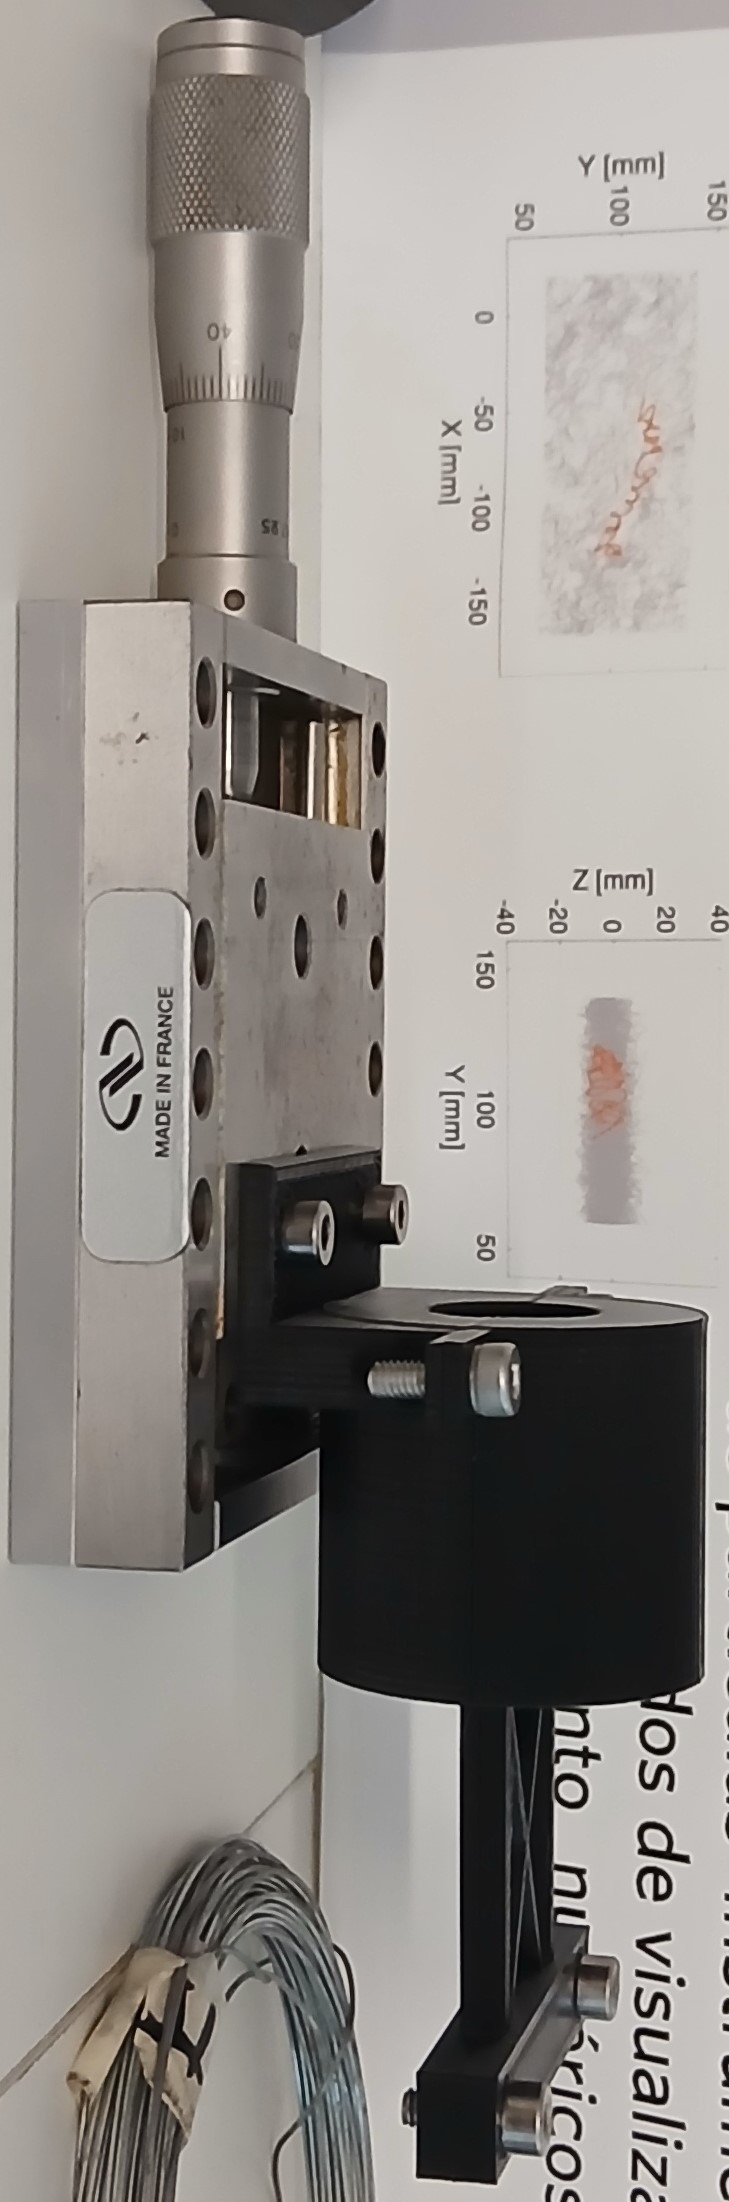
\includegraphics[height=250pt]{Figures/21_04_2025/Vista_3_4_impresa.jpg}
				\captionsetup{width=0.8\textwidth}
				\subcaption{Vista 3/4.}
			\end{subfigure}
		\end{minipage}
	\caption{Fotos del nuevo modelo de carcasa ya impreso y conectado al tornillo micrométrico.} % k 
	\label{fig:}
\end{figure}

Faltaría conseguir tuercas M4 para terminar de cerrar ambas mitades de la carcasa.

\subsection*{Conectar el tornillo a un perfil.}

\begin{figure}
	\centering
	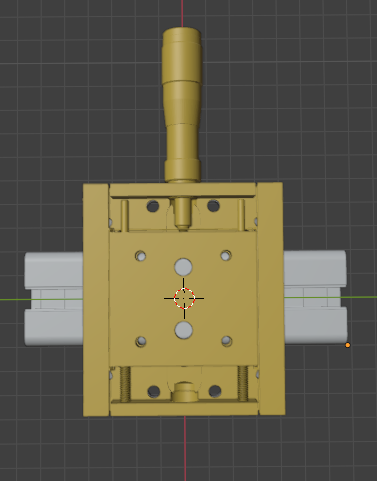
\includegraphics[width=0.7\linewidth]{Figures/21_04_2025/Vista_frontal_tornillo_perfil}
	\caption{}
	\label{fig:vistafrontaltornilloperfil}
\end{figure}


\begin{figure}
	\centering
	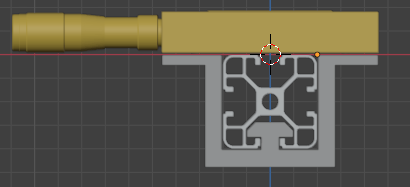
\includegraphics[width=0.7\linewidth]{Figures/21_04_2025/Vista_lateral_tornillo_perfil}
	\caption{}
	\label{fig:vistalateraltornilloperfil1}
\end{figure}

\begin{figure}
	\centering
	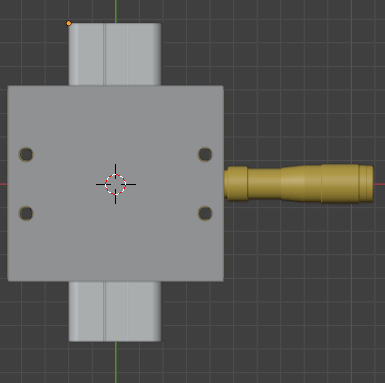
\includegraphics[width=0.7\linewidth]{Figures/21_04_2025/Vista_trasera_tornillo_perfil}
	\caption{}
	\label{fig:vistatraseratornilloperfil}
\end{figure}

\begin{figure}
	\centering
	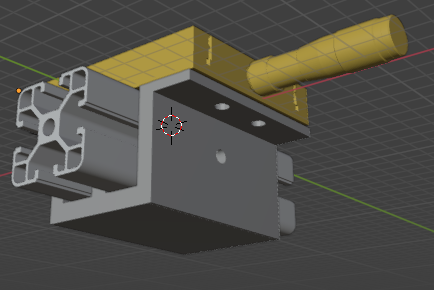
\includegraphics[width=0.7\linewidth]{Figures/21_04_2025/Vista_3_4_tornillo_perfil1}
	\caption{}
	\label{fig:vista34tornilloperfil1}
\end{figure}